% thesis.tex
%
% This file is root file for an example thesis written using the
% University of Wisconsin-Madison LaTeX Style file.
%
% It is provided without warranty on an AS IS basis.


%=====================================================================
% Document Style
%=====================================================================
% Choose only one of the following document classes:
%
% for a 12 Point UW PhD Thesis without Margin Check
\documentclass[12pt]{withesis}
%
% for a 10 Point UW PhD Thesis with Margin Check
%\documentclass[10pt,margincheck]{withesis}
%
% The margincheck option flags lines which overflow their hbox with a black
%  box at the end of the line.  This usually (but not always) indicates a
%  margin violation on the right margin.  Left margin violations aren't
%  indicated and if the margin violation is large enough, there isn't room
%  for the black box to be visiable.  
%
% This option can be also used in conjunction with the msthesis option.
%
% or for a 12 Point UW Masters Thesis
%\documentclass[12pt,msthesis]{withesis}
%
% or for a 10 Point UW Masters Thesis
%\documentclass[10pt,msthesis]{withesis}
%
% The msthesis option changes the page margins from 1" all around
% (the PhD format) to 1.25" left and 1" remaining margins (MS format).
% The defaults for degree and thesis are changed to be MS and thesis.
% These defaults can be overridden if the margins for the MS thesis
% are desired for other documents.

% To include optional packages, use the \usepackage command.
%  The package epsfig is used to bring in the Encapsulated PostScript
%    figures into the document.
%  The package times is used to change the fonts to Times Roman; however
%    because the times typewriter font looks odd, the original LaTeX
%    Computer Modern font is kept for the typewriter font using
%      \renewcommand{\ttdefault}{cmtt}
%    Note that Times Roman is a PostScript font and therefore, the document
%    cannot be correctly viewed from the *.dvi file.  It should be converted
%    to a *.ps file first and then viewed with a PostScript previewer...
\usepackage{epsfig}
\usepackage{graphicx}
\usepackage{times}
\renewcommand{\ttdefault}{cmtt}

%========================================================================
%  Draft Control Commands:
%========================================================================
%
% \psdraft causes the \psfig or \epsfig commands to draw a box and label
% the box with the postscript file name instead of reading in the full
% postscript figure.  This can save time and toner when printing drafts.
%
%\psdraft
%
%
% \psfull causes the inclusion of the postscript figures.
%\psfull
%
%
%\pagestyle{thesisdraft} causes the footer text to become:
% DRAFT: Do Not Distribute        <time><Date>        <input file name>
%
%\pagestyle{thesisdraft}
%
%\pagestyle{thesis} causes the header and footers to be the correct format
%
\pagestyle{thesis}
%
%
%  The page margins can be marked with a post-script box using the
%  \draftmargins command.  This command uses dvips's end-of-page hook
%  This is only visible in the *.ps file (NOT the *.dvi file)!
%
%\draftmargins
%
%
%  The word ``DRAFT'' can be diagonally printed across the page using
%  the \draftscreen command.  This command uses dvip's beginning-of-page
%  hook.  This is only visible in the *.ps file (NOT the *.dvi file)!
%
%\draftscreen


%=======================================================================
% Remove the following lines if appendix tables or figures are present.
% The suppress writing the auxiliary information which appears in the
% list of tables or list of figures.
%
\noappendixtables                % Don't have appendix tables
\noappendixfigures               % Don't have appendix figures


%=======================================================================
% End of Preamble, start of document
%


\begin{document}

% Choose your bibliography style
% plain is the basic style, others include ieeetr, siam, asm, etc
\bibliographystyle{plain}


% prelude.tex
%   - titlepage
%   - dedication
%   - acknowledgments
%   - table of contents, list of tables and list of figures
%   - nomenclature
%   - abstract
%============================================================================


\clearpage\pagenumbering{gobble}  % This makes the page numbers Roman (i, ii, etc)



% TITLE PAGE
%   - define \title{} \author{} \date{}
\newcommand{\actualtitle}{Zimbra 8 High Availability on Ubuntu 12.04}
\title{\actualtitle}
\newcommand{\actualauthor}{Adri\'an Gibanel L\'opez}
\author{\actualauthor}
\date{2013}
%   - The default degree is ``Doctor of Philosophy''
%     (unless the document style msthesis is specified
%      and then the default degree is ``Master of Science'')
%     Degree can be changed using the command \degree{}
\degree{M\`aster en Enginyeria de Programari Lliure}
%   - The default is dissertation, unless the document style
%     msthesis was specified in which case it becomes thesis.
%     If msthesis is specified for the MS margins, you can
%     still have a dissertation if you specify \disseration
%\disseration
%   - for a masters project report, specify \project
%\project
%   - for a preliminary report, specify \prelim
%\prelim
%   - for a masters thesis, specify \thesis
\masterthesis
%   - The default department is ``Electrical Engineering''
%     The department can be changed using the command \department{}
\department{Dept. d'Informatica i Enginyeria Industrial}
%   - once the above are defined, use \maketitle to generate the titlepage
\advisorname{Josep Maria Rib\'o Balust}
\advisortitle{Professor}
\newdateformat{udlthesisdate}{\monthname[\THEMONTH] \THEYEAR}

% Title - BEGIN
\let\textquotedbl="
\pagestyle{empty}~

~

~

\begin{center}
{\LARGE \title{}}
\par\end{center}{\LARGE \par}

~
\begin{center}

\includegraphics[scale=0.4]{img/udl}
\par\end{center}
~

~

\begin{center}
{\large Universitat de Lleida}
\par\end{center}{\large \par}

\begin{center}
{\large Escola Polit\`ecnica Superior}
\par\end{center}{\large \par}

\begin{center}
{\large M\`aster en Enginyeria de Programari Lliure}
\par\end{center}{\large \par}

%\begin{center}
%{\large Dept. d'Informatica i Enginyeria Industrial}
%\par\end{center}{\large \par}


~

~
\begin{center}
{\large Treball de final de m\`aster}
\par\end{center}{\large \par}


~
\begin{center}
{\large \textbf{Zimbra 8 High Availability on Ubuntu 12.04}}
\par\end{center}{\large \par}


~

~


\hfill {\large Autor/a: Adri\'an Gibanel L\'opez}
\par{\large \par}

~

\hfill {\large Director/s: Josep Maria Rib\'o Balust}
\par{\large \par}

~

\hfill {\large Setembre 2013}
\par{\large \par}

\newpage

Copyright (c) 2013 Adrian Gibanel Lopez.

Permission is granted to copy, distribute and/or modify this document

under the terms of the GNU Free Documentation License, Version 1.3

or any later version published by the Free Software Foundation;

with no Invariant Sections, no Front-Cover Texts, and no Back-Cover
Texts.

A copy of the license is included in the section entitled \textquotedbl{}GNU

Free Documentation License\textquotedbl{}.

\newpage


% Title - END

% DEDICATION
\newpage
\null\vfil
\begin{center}
To the bTactic crew
\end{center}
\par\vfil\newpage

% ACKNOWLEDGMENTS

\chapter*{ACKNOWLEDGMENTS}
%\doublespace
I acknowledge Richard M. Stallman for his personal commitment to the free software movement.
\par\newpage




% ABSTRACT

\section* {ABSTRACT}
             \thispagestyle{empty}
                  \addtocounter{page}{-1}
                \begin{center}
                  {\bf\expandafter\uppercase\expandafter{\actualtitle}}\\
                  \vspace{12pt}
                  \actualauthor \\
                  \vspace{12pt}
                  Under the supervision of Professor Josep Maria Rib\'o Balust\\
                  At the Universitat de Lleida
                \end{center}

% abstract.tex
%
% This file has the abstract for the withesis style documentation
%
% Eric Benedict, Aug 2000
%
% It is provided without warranty on an AS IS basis.

\noindent       % Don't indent this paragraph.
The purpose of this master thesis is to design and test the setup of a Zimbra 8 Open Source Edition (OSE) High Availability System (HA) in Ubuntu 12.04.


\vspace*{0.5em}
\noindent       % Don't indent this paragraph.
A HA system has been proposed and tested in a laboratory environment. Its setup has been documented in its all length.

\vspace*{0.5em}
\noindent       % Don't indent this paragraph.
The master thesis shows that thanks to some minor modifications to Zimbra OSE core and thanks to freely available Open Source HA software one can achieve a HA Zimbra OSE system.

\vspace*{0.5em}
\noindent       % Don't indent this paragraph.
The proposed HA Zimbra OSE system can be improved in many ways and the author suggests several ways of doing so.

\pagestyle{headings}

% CONTENTS, TABLES, FIGURES
\tableofcontents
%\listoftables
\listoffigures
\newpage

\clearpage\pagenumbering{arabic} % This makes the page numbers Arabic (1, 2, etc)
                % Title page, abstract, table of contents, etc
% Problem description


\chapter{Introducing Zimbra High Availability}
This thesis was written to reflect the state of the art in High Availability methods for Zimbra Open Source Edition.  

\section {High Availability}
High availability is a system design approach and associated service implementation that ensures that a prearranged level of operational performance will be met during a contractual measurement period.

One of the most common high availability examples are web servers. Two web servers share the same information thanks to a shared storage. If one of the web servers fails to serve pages the other server can reclaim its primary role and shot the other node in the head (stonith) so that it can serve pages instead of the original primary node. The amount of time since the detection of the first server failure to its reestablishment is denoted as downtime. A contract for High Availability might stipulate that in a month time web servers service might be in downtime status for no more than five minutes.

High Availability, or HA as it is abbreviated, refers to the availability of resources in a computer system, in the event of component failures in the system. This can be achieved in a variety of ways, either with custom and redundant hardware to ensure availability or with software solutions using off-the-shelf hardware components.

The former class of solutions provide a higher degree of availability, but are significantly more expensive than the latter. This has led to the popularity of the latter class, with almost all vendors of computer systems offering various HA products. Typically, these products endure single points of failure in the system. (\cite{TaskForceHA})

As an example for more expensive systems we can mention OVH.co.uk web hosting service which uses more than 1,000 servers not only for ensuring high availability but also for dealing with high loads of visitor's queries. SQL servers seem to achieve high availability by using several RAID-1 (mirror) hard disks.

These HA systems usually ensure that a prearranged level of operational performance will be met during a contractual measurement period. (\cite{WikipediaHA})

High availability systems typically operate 24x7 and usually require built-in redundancy to minimize the risk of downtime due to hardware and/or telecommunication failures. 

Availability can be measured relative to "100\% operational" or "never failing." A widely-held but difficult-to-achieve standard of availability for a system or product is known as "five 9s" (99.999 percent) availability. (\cite{BCMHA})

From now on high availability will be refered as HA.

\section {Vmware Zimbra OSE}
VMware Zimbra is a complete email, address book, calendar and tasks solution that can be accessed from the Zimbra Web Client, Zimbra Desktop offline client, Outlook and a variety of other standards-based email clients and mobile devices. It can be deployed as a traditional binary install on Linux, or as a software virtual appliance, commonly referred to as Zimbra appliance.

Among the Zimbra Collaboration Server (ZCS) versions this thesis will approach the ZCS Open Source Edition also known as Zimbra OSE.

Vmware Zimbra OSE will be referred most of the times as Zimbra.

For more information about Vmware Zimbra you can visit: \cite{ZimbraLearn}.

\section {Vmware Zimbra OSE High Availability}
Zimbra OSE High Availability is a project which attempts to attain HA to each one of the Zimbra Collaboration Server components so that the risk of downtime due to hardware and/or telecommunication failures is minimized. High availability is usually implemented using High Availability software aimed at Gnu/Linux originally which is adapted to the Zimbra OSE setup.


\section{\label{sec:history}History}

Prior documentation about Zimbra High Availability was written with Zimbra 6 version in mind which is devoted to work (among others) in Ubuntu 8.04 64 bit. That documentation was based on Gnu/Linux High Availability software (heartbeat) which is no longer used for High Availability purposes nowadays.

To the best of the author's knowledge there is no updated documentation on how to setup this system.

On September 13th, 2012 Vmware announced Zimbra 8 which could be run in Ubuntu 12.04 (\cite{VmwareZimbra8Announce}).

\section {Main thesis topic}
The main topic of this thesis is: \\
\textit{Design and test the setup of a Zimbra 8 High Availability System in Ubuntu 12.04 and write a detailed report of this setup procedure.}

\section {Chosen technologies and solution}
We have decided to use the following proved open source HA technologies:\\ Corosync, Distributed Replicated Block Device (DRBD), OCF, and Pacemaker.

Corosync is a software meant to synchronize configuration files. Synchronize configuration files in a cluster is essential because all the cluster members have to share the same information and knowledge of the other cluster members. DRBD allows us to share a common storage between hosts as if a network RAID-1 hard disk it was. Finally, in order to setup and manage the whole cluster we will use Pacemaker cluster which uses OCF scripts as Cluster control scripts.

The reason for using these technologies is because they are the best well known and most used open source HA technologies. They have supersesed old technologies like heartbeat which we mentioned in \textbf{section {\ref{sec:history} History}}.

A set of virtual machines will be used to setup Zimbra 8 and Ubuntu 12.04 HA system. The neccessary steps to carry out this setup are: Setup network in both hosts, setup DRBD, initial Pacemaker setup, corosync installation, pacemaker installation, corosync setup, startup script disabling, DRBD script boot disabling, Pacemaker final setup, Pacemaker case of use tests.

This report describes in detail the setup procedure of each of these steps.

\section {Notation remarks}
Zimbra will be run in two \textit{servers} in our solution. These servers will be refered to as \textit{virtual servers} when we take the point of view of Virtualbox or virtualization point of view as in section \textbf {\ref{sec:virtualbox-implementation} Virtualbox implementation}.

When the HA system will be described these same servers will be refered to as \textit{nodes} as this is the way most HA software refer to their own cluster machines.

\section {Structure of the document}

Chapter 2 explains the high availability system that will be tested through the thesis.

Chapters 3 to 12 explain the detailed setup procedure of each element that constitutes the final system: \textit{\ref{chap:ha-schema} - High availability schema},
\textit{\ref{chap:operating-system-installation} - Operating System installation},
\textit{\ref{chap:network-setup} - Network setup},
\textit{\ref{chap:zimbra-installation} - Zimbra installation},
\textit{\ref{chap:drbd-setup} - DRBD Setup},
\textit{\ref{chap:zimbra-drbd-startup-script-disabling} - Zimbra and DRBD Startup Script Disabling},
\textit{\ref{chap:corosync-setup} - Corosync Setup},
\textit{\ref{chap:zimbra-ocf} - Zimbra OCF Resource Agent development},
and
\textit{\ref{chap:pacemaker-setup} - Pacemaker Setup}.
Final system is a Zimbra OSE High Availability system with two servers.

We learn how to manage our new High Availability system thanks to the \textit{\ref{chap:ha-system-management} - High Availability System Management} chapter.

Finally both conclusions and some of the ways this thesis can be improved are described in \textit{\ref{chap:conclusions-and-future-work}} chapter.

                  % Chapter 1
% HA Schema


\chapter{High availability schema}
\label{chap:ha-schema}
This chapter explains the high availability system that will be tested through the Thesis. 

\section {Purpose}
The proposed HA system is an Active/passive configuration. An Active/passive cluster provides a fully redundant instance of each node, which is only brought online when its associated primary node fails (\cite{HAClusterNodeConfigurations}).

In our case, the primary node will act as the active server and it will provide Zimbra services such as web server, smtp, imap, etc. The secondary node will be idle just waiting for the primary node to fail and bring Zimbra services online when that event happens. In addition the secondary node also mirrors Zimbra data partition in the background thanks to DRBD.

\section {Main schema}
There are two servers which we will be named as the primary one and the secondary one. They are linked by means of two connections: The service and the communication link.

The service link is the main network interface which is connected via a normal switch. It will serve content to the final users. The communication link, which is used for the cluster management and synchronization is done via a crossover cable.

We can see the main schema, where we have added two final clients at figure \ref{fig:main-schema}.

\begin{figure}
  \centering
    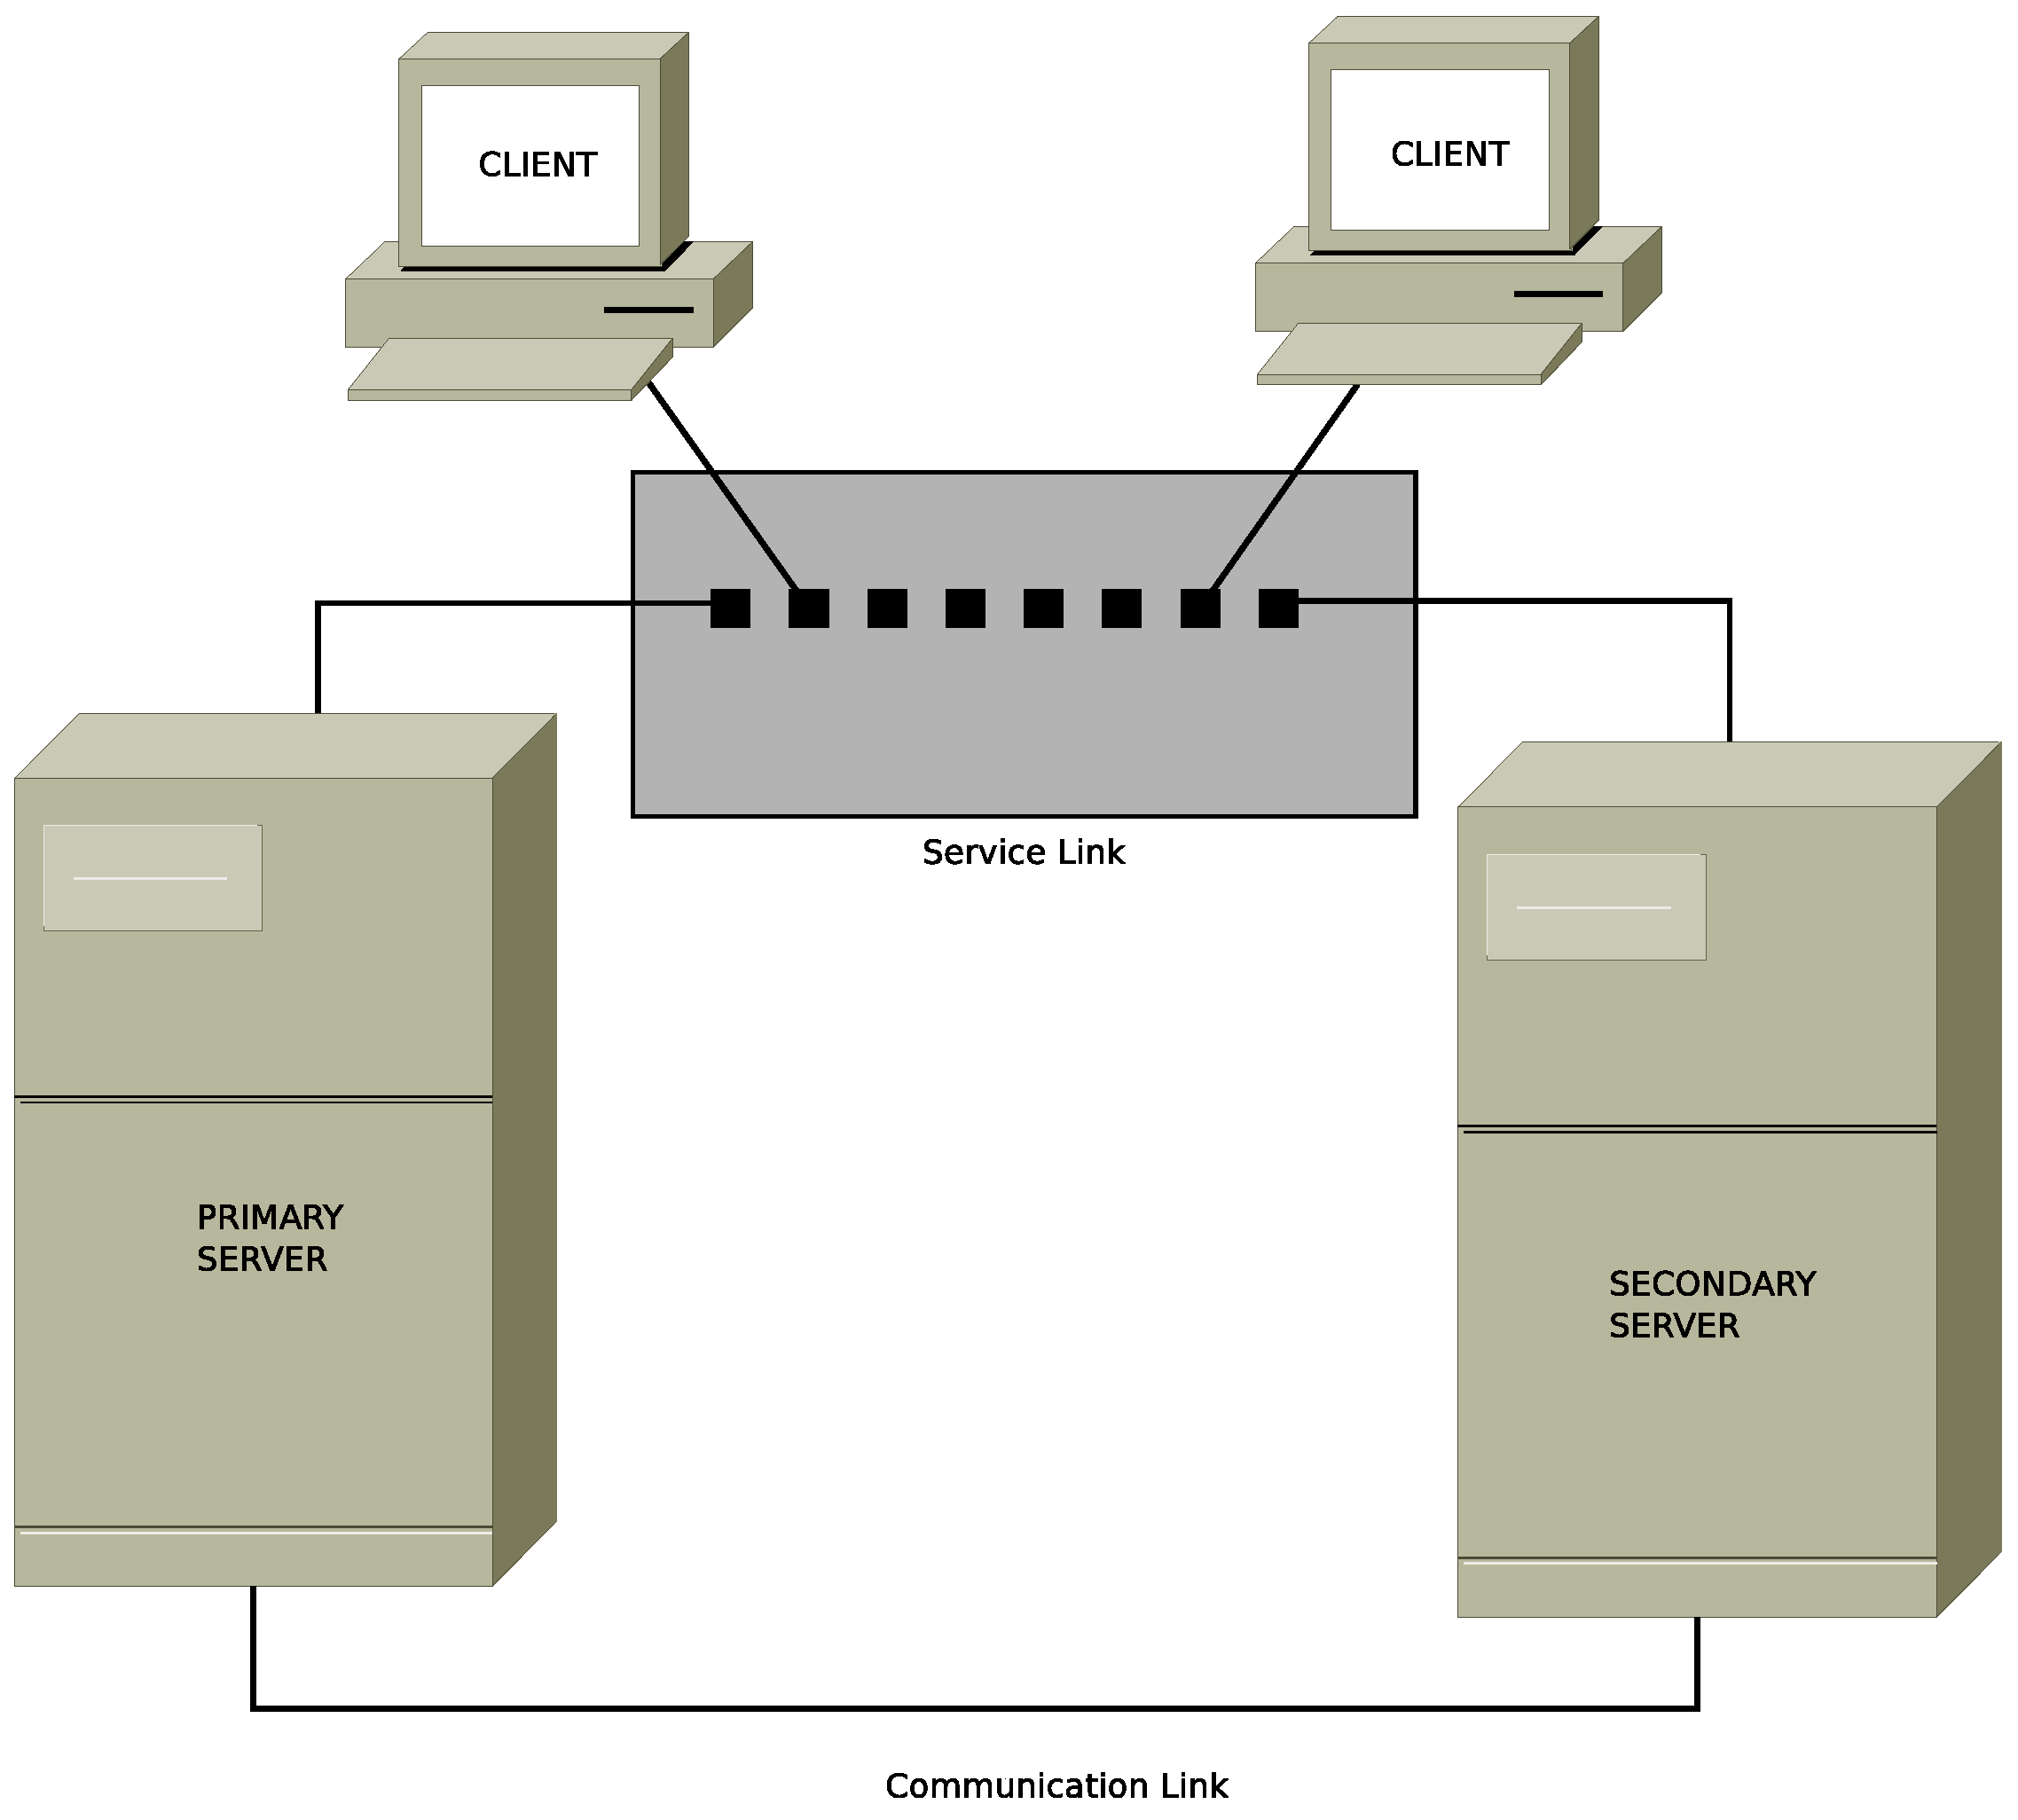
\includegraphics[width=0.8\textwidth]{img/ha_main_schema.eps}
  \caption{High Availability main schema}
  \label{fig:main-schema}
\end{figure}

\section {Primary server}
\subsection {Specifications}
The primary server specifications are as follow:
\begin{itemize}
  \item RAM: 4 GB
  \item Hard disk: 100 GB
  \item Processor: 2 x 2,40 Ghz
\end{itemize}

\section {Secondary server}
\subsection {Specifications}
The primary server specifications are as follow:
\begin{itemize}
  \item RAM: 4 GB
  \item Hard disk: 100 GB
  \item Processor: 2 x 2,40 Ghz
\end{itemize}

\section {\label{sec:virtualbox-implementation}Virtualbox implementation}
\subsection {Introduction}
Although in production environments High Availability systems are implemented in Physical servers or highly optimized virtualized servers, we are going to use Oracle VM Virtualbox software to emulate the described system. This section summarizes how to create both virtual machines and link them.

\subsection {\label{subsec:primary-virtual-machine-creation}Primary Virtual Machine creation}
We click on \textit{Machine} menu and select \textit{New} option. The Create Virtual Machine wizard will appear.

\subsubsection {Name and operating system}
\begin{itemize}
  \item Name: PrimaryZimbraHA
  \item Type: Linux
  \item Ubuntu (64 bit)
\end{itemize}

\subsubsection {Memory size}
Zimbra needs: 2048 MB as a minimum.
\subsubsection {Hard drive}
We select \textit{Create a virtual hard drive now}, \textit{Virtualbox Disk Image} as the hard drive file type, Dynamically allocated (so that the hard drive file only uses space as it fills up).

We leave the default File location and select hard disk size as 110 GB which is quite bigger than the strictly needed for our HA system.

\subsection {\label{subsec:service-link-primary}Service link network on Primary Virtual Machine}
We select \textit{PrimaryZimbraHA} virtual machine and click on \textit{Machine} menu and then in \textit{Settings} option. We will make sure we are in \textit{Network} section.

We will use default \textit{Adapter 1} for service link. We are going to summarize its setup:
\begin{itemize}
  \item Attached to: \textit{Internal Network}
  \item Name: ZimbraHAService
\end{itemize}

Finally we click on OK for saving changes.

\subsubsection {Secondary Virtual Machine creation}
In order to create secondary virtual machine we can either repeat the same steps as in \textbf{\ref{subsec:primary-virtual-machine-creation} Primary Virtual Machine creation}. Or we can make a linked clonation of the original machine. We will describe the latter option.

We select PrimaryZimbraHA virtual machine and then in \textit{Machine} menu we select \textit{Clone} option.

\textbf{New machine name}
\begin{itemize}
  \item New machine name: SecondaryZimbraHA
  \item Reinitialize the MAC address of all network cards: Checked
\end{itemize}

We select \textit{Linked clone} as Clone type.

Finally we click on \textit{Clone} button so that cloning is performed.

\subsection {Service link network on Secondary Virtual Machine}
As we did in subsection \textbf{\ref{subsec:service-link-primary} Service link network on Primary Virtual Machine} we select \textit{SecondaryZimbraHA} virtual machine and click on \textit{Machine} menu and then in \textit{Settings} option. We will make sure we are in \textit{Network} section.

We will use default \textit{Adapter 1} for service link. We are going to summarize its setup:
\begin{itemize}
  \item Attached to: \textit{Internal Network}
  \item Name: \textit{ZimbraHAService}
\end{itemize}

If we have cloned the virtual machine settings might be correct by default.

Finally we click on OK for saving changes.

\subsection {Communication link}
For both PrimaryZimbraHA and SecondaryZimbraHA virtual machines we will perform a very similar operation than the one done in subsection \textbf{\ref{subsec:service-link-primary} Service link network on Primary Virtual Machine}.

But now we make sure that we \textit{Adapter 2} is enabled as an \textit{Internal Network} which name is \textit{ZimbraHACommunication}.

\subsection {NAT link}
In order to make installation easier we will enable \textit{Adapter 3} in both virtual machines so that it can use the host Internet in order to fetch packages and perform post installation setup.

Similarly to subsection \textbf{\ref{subsec:service-link-primary} Service link network on Primary Virtual Machine} we make sure that \textit{Adapter 3} is enabled and that it's attached to NAT.

\subsection {Email client Virtual Machine}
A Virtual Machine whose only purpose is to test HA from a service link point of view might be added if needed. We're not to cover the installation and its setup here. We will just mention its network setup is similar to PrimaryZimbraHA and SecondaryZimbraHA but removing the second interface which serves for communication link and that, of course, doesn't make sense in an Email client VM.
% Operating System installation


\chapter{Operating System installation}
This chapter explains the Operating System installation.

\section {Introduction}
The reason why Ubuntu 12.04 in its 64bit mode is used is because is one of the official supported Operating System for Zimbra 8 versions. We denote an external DRBD metadata as DRBD-Meta-Disk. We can understand it is an special partition that helps DRBD system to track changes between synchronised partitions between both primary and secondary nodes. We can find a more accurate definition at Linbit site: \cite{LinbitDRBDInternals}.

\section {Ubuntu 12.04 64 bit minimal}
In order to track all the requisites and just install what the high availability system needs we will use an Ubuntu minimal disk for installation. These disks can be downloaded from \cite{UbuntuMinimalDisk}.

The used download was: \textit{Ubuntu 12.04 "Precise Pangolin" Minimal CD} from the \textit{64-bit PC (amd64, x86\_64)} section. 

\section {TODO: steps1}
\section {Partitioning}
Both virtual machines will have the same partitioning scheme. Both virtual machines have two hard disks.
Assuming a 1.8 Terabyte hard disk in order to setup DRBD-Meta-Disk there's enough with 59 megabytes. We will be on the safe side and setup it with a 150 megabytes size. In order to safe calculate other DRBD meta disk partitions we can check \cite{LinbitDRBDInternals}.

Hard Disk 1:
\begin{verbatim}
sda1 / 10GB ext4
sda2 DRBD-Meta-Disk 150MB ext4
sda3 (LVM Partition + Free space for LVM snapshots)
\end{verbatim}

sda3 contains a LVM's Volume Group named zimbra.
This Volume Group has a Logical Volume named zimbra also which doesn't ocuppy the full Volume Group space. The reason is that we reserver some space for snapshots when doing backups.

In our case we did:
\begin{verbatim}
VG zimbra: 1,8 TB

  LV zimbra: 1770 GB
  Free space: 30 GB
\end{verbatim}


Hard Disk 2:
\begin{verbatim}
sdb1 / 2 GB SWAP
\end{verbatim}

% Network Setup


\chapter{Network setup}
\label{chap:network-setup}
This chapter explains the network setup.

\section {Network schema}
We can just check the High Availability main schema (figure \ref{fig:main-schema}) where network has been already described. There are two networks. The service link is the main network interface for serving content to the final users. The communication link, which it's used for the cluster management and syncronisation is done via a crossover cable.

\section {VirtualBox Network Implementation}

In order to implement this Network schema in VirtualBox the service link will be setup by the first virtual network card in each virtual machine. Both of tese virtual network card will be setup in bridge mode so that an actual switch serve them. The communication link will be setup by the second virtual network card in each virtual machine connected to a VirtualBox private network, that means that they will be connected via a virtual switch given by Virtualbox which it's isolated from other networks.

TODO: Add VirtualBox Network figure.

\section {Network setup}

\subsection {Primary server}
\subsubsection {Service link}
Primary server's Service link network setup consists of a Class C configuration where the network card address is 192.168.1.201, as per being a Class C its netmask is 255.255.255.0 and thus its broadcast is 192.168.1.255. As a gateway it will be using the first network address in the network range which it's 192.168.1.1.

\begin{verbatim}
auto eth0
iface eth0 inet static
        address 192.168.1.201
        netmask 255.255.255.0
        broadcast 192.168.1.255
        gateway 192.168.1.1
\end{verbatim}

\subsubsection {Communication link}
Primary server's Communication link network setup consists of a Class C configuration where the network card address is 10.0.2.201, as per being a Class C its netmask is 255.255.255.0 and thus its broadcast is 10.0.2.255. As a gateway it will be using the first network address in the network range which it's 10.0.2.1.

\begin{verbatim}
auto eth0
iface eth0 inet static
        address 10.0.2.201
        netmask 255.255.255.0
        broadcast 10.0.2.255
        gateway 10.0.2.1
\end{verbatim}
\subsection {Secondary server}
\subsubsection {Service link}
Secondary server's Service link network setup consists of a Class C configuration where the network card address is 192.168.1.202, as per being a Class C its netmask is 255.255.255.0 and thus its broadcast is 192.168.1.255. As a gateway it will be using the first network address in the network range which it's 192.168.1.1.

\begin{verbatim}
auto eth0
iface eth0 inet static
        address 192.168.1.202
        netmask 255.255.255.0
        broadcast 192.168.1.255
        gateway 192.168.1.1
\end{verbatim}

\subsubsection {Communication link}
Secondary server's Communication link network setup consists of a Class C configuration where the network card address is 10.0.2.202, as per being a Class C its netmask is 255.255.255.0 and thus its broadcast is 10.0.2.255. As a gateway it will be using the first network address in the network range which it's 10.0.2.1.

\begin{verbatim}
auto eth0
iface eth0 inet static
        address 10.0.2.202
        netmask 255.255.255.0
        broadcast 10.0.2.255
        gateway 10.0.2.1
\end{verbatim}

\section {Firewall}

TODO: Describe firewall. Ports that have been left opened.



% Zimbra installation


\chapter{Zimbra installation}
\label{chap:zimbra-installation}
This chapter explains the Zimbra OSE installation.

\section {Zimbra 8.0.4 for Ubuntu 12.04}
Zimbra 8.0.4 for Ubuntu 12.04 in form of a tar.gz file was downloaded from \cite{Zimbra8Download}.
Once downloaded is advised to check its md5sum. Finally we untar it and cd into the untarred directory.

\section {Install script launch}



% DRBD Setup


\chapter{DRBD Setup}
This chapter explains the DRBD Setup.

\section {Introduction}
DRBD is a system that let us mirror a block device via an assigned device. DRBD can be understood as network based raid-1 and it's used in high availability (HA) clusters (\cite{LinbitDRBDWhatIs}).
We're using DRBD to mirror the block device where Zimbra files will be stored on.

\section {Requirements}
We will install DRBD packages for the Ubuntu 12.04 system thanks to the following command:
\begin{verbatim}
sudo apt-get install drbd8-utils
\end{verbatim}
.



\section {DRBD Resource config}
\textbf{To be performed in both servers}.

We will backup main drbd configuration file:
\begin{verbatim}
cp /etc/drbd.conf /etc/drbd.conf.orig
\end{verbatim}
.

We then need to edit:
\begin{verbatim}
/etc/drbd.conf
\end{verbatim}
so that it has:
\begin{verbatim}
resource zimbradata {
  protocol C;
  incon-degr-cmd "halt -f";
  startup {
    degr-wfc-timeout 120; # 2 min
  }
  disk {
    on-io-error detach;
  }
  net {
  }
  syncer {
    rate 10M;
    group 1;
    al-extents 257;
  }
  on zhatest-01.dominio.com {
    device /dev/drbd0;
    disk /dev/zimbra/zimbra;
    address zhatest-01-comm-ip:7788;
    meta-disk /dev/sda2[0];
  }
  on zhatest-02.dominio.com {
    device /dev/drbd0;
    disk /dev/zimbra/zimbra;
    address zhatest-02-comm-ip:7788;
    meta-disk /dev/sda2[0];
  }
}
\end{verbatim}
.

TODO: Explain drbd.conf contents and what they mean more or less.

If we want to modify our drbd.conf to increase sync rate, synchronised devices or any other settings we can check documentation at \cite{LinbitDRBDdrbdconf}.

\section {Start DRBD module}
\textbf{To be performed in both servers}.
\begin{verbatim}
modprobe drbd
\end{verbatim}
.
\section {Metadata disk initialisation}
\textbf{To be performed in both servers}.
We make sure the metadata partition does not have any prior metadata signature.
\begin{verbatim}
dd if=/dev/zero of=/dev/sda2 bs=1K count=100
\end{verbatim}
And we create the zimbradata metadata partition:
\begin{verbatim}
drbdadm create-md zimbradata
\end{verbatim}
.

\section {Primera sincronizaci\'on DRBD}
\textbf{To be performed in both servers}.
\begin{verbatim}
drbdadm up all
\end{verbatim}
where we shouldn't find any incorrect hostname errors.
TODO: Rewrite last line.

We will be asked about usage survey, we just reply that we don't want to participate by saying 'no'.

\textbf{To be performed in Primary server only}.
\begin{verbatim}
drbdadm -- --do-what-I-say primary all
drbdadm -- connect all
\end{verbatim}
.

If we happen to find a \textit{net-config disconnect first} error we can safely ignore it.

In order to check DRBD first synchronisation status we need to check /proc/drbd file with:
\begin{verbatim}
cat /proc/drbd
\end{verbatim}
which will output something like:
\begin{verbatim}
version: 0.7.20 (api:77/proto:74)
SVN Revision: 1743 build by <a href="mailto:phil@mescal">\
phil@mescal</a>, 2005-01-31 12:22:07
0: cs:SyncSource st:Primary/Secondary ld:Consistent
ns:13441632 nr:0 dw:0 dr:13467108 al:0 \
bm:2369 lo:0 pe:23 ua:226 ap:0
[==>..............] sync'ed: 3.1% (7000/7168)M
finish: 1:14:16 speed: 2,644 (2,204) K/sec
1: cs:Unconfigured
\end{verbatim}
.

We must wait for the process to finish in order to continue.







%\include{Initial Pacemaker Setup}
%\include{Corosync installation}
%\include{Pacemaker installation}
%\include{Corosync setup}
%\include{Startup script disabling}
%\include{DRBD Script Boot disabling}
%\include{Pacemaker final setup}
%\include{Pacemaker case of use tests}
     
%\include{figs}
%\include{bibs}

%\bibliography{refs}              % Make the bibliography

\begin{appendices}               % Start of the Appendix Chapters.  If there is only
                                 % one Appendix Chapter, then use \begin{appendix}
%\include{code}                   % Including computer code listings
%\include{bibref}                 % a BibTeX reference
%\include{math}                   % Complex Equations from the UW Math Department
%\include{acro}                   % A discussion on generating PDF files.
\end{appendices}                 % End of the Appendix Chapters.  ibid on \end{appendix}
%\include{vita}                  % Optional Vita, use \begin{vita} vita text \end{vita}
\end{document}
